\documentclass{article}
\usepackage{parskip}
\usepackage{pdfpages}
\usepackage[margin=.6in]{geometry}
\begin{document}
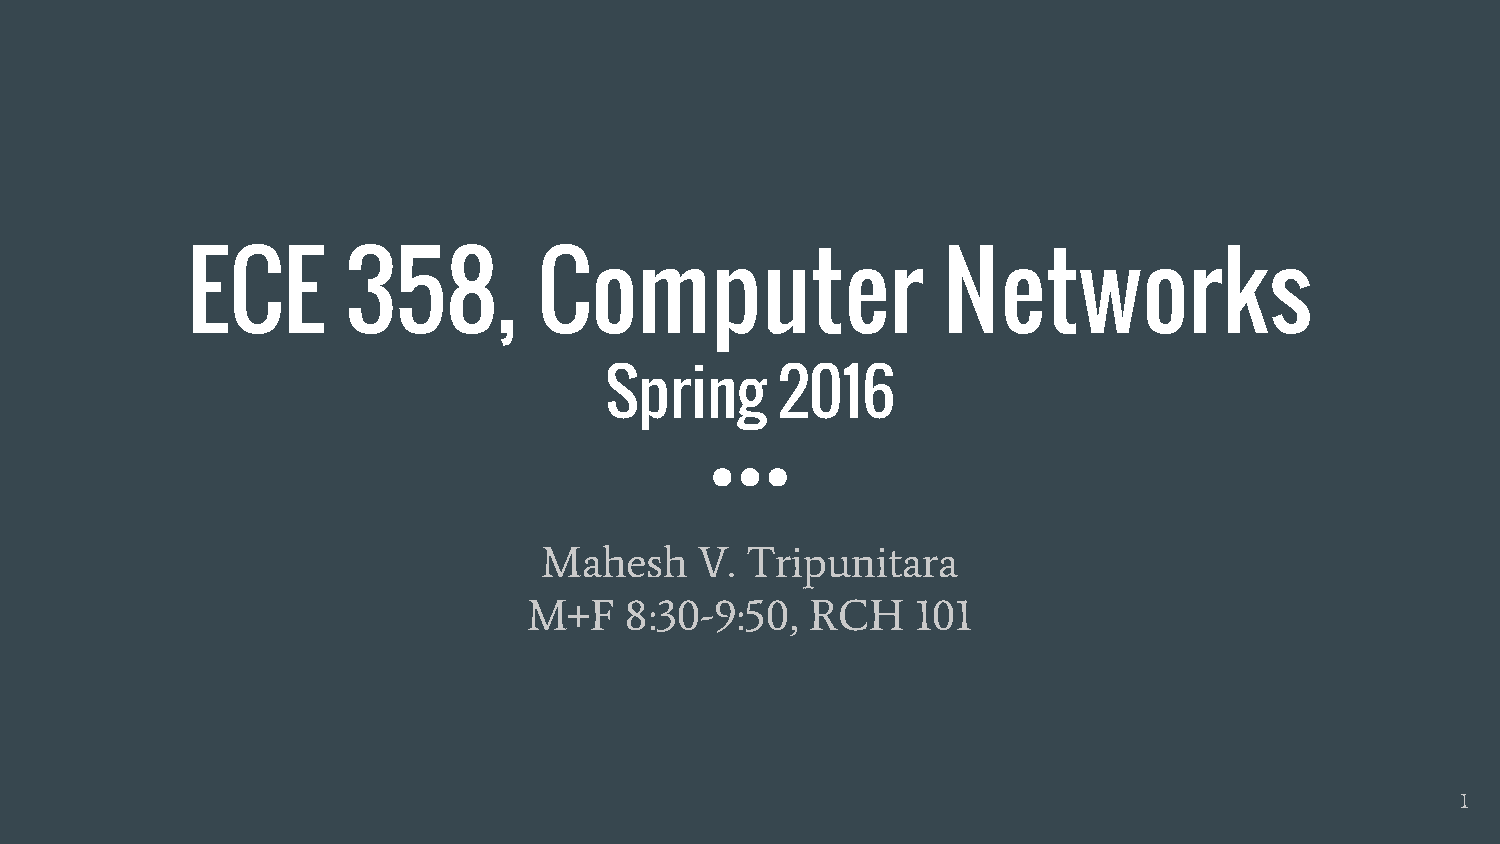
\includepdf[page=1-14]{slides.pdf}

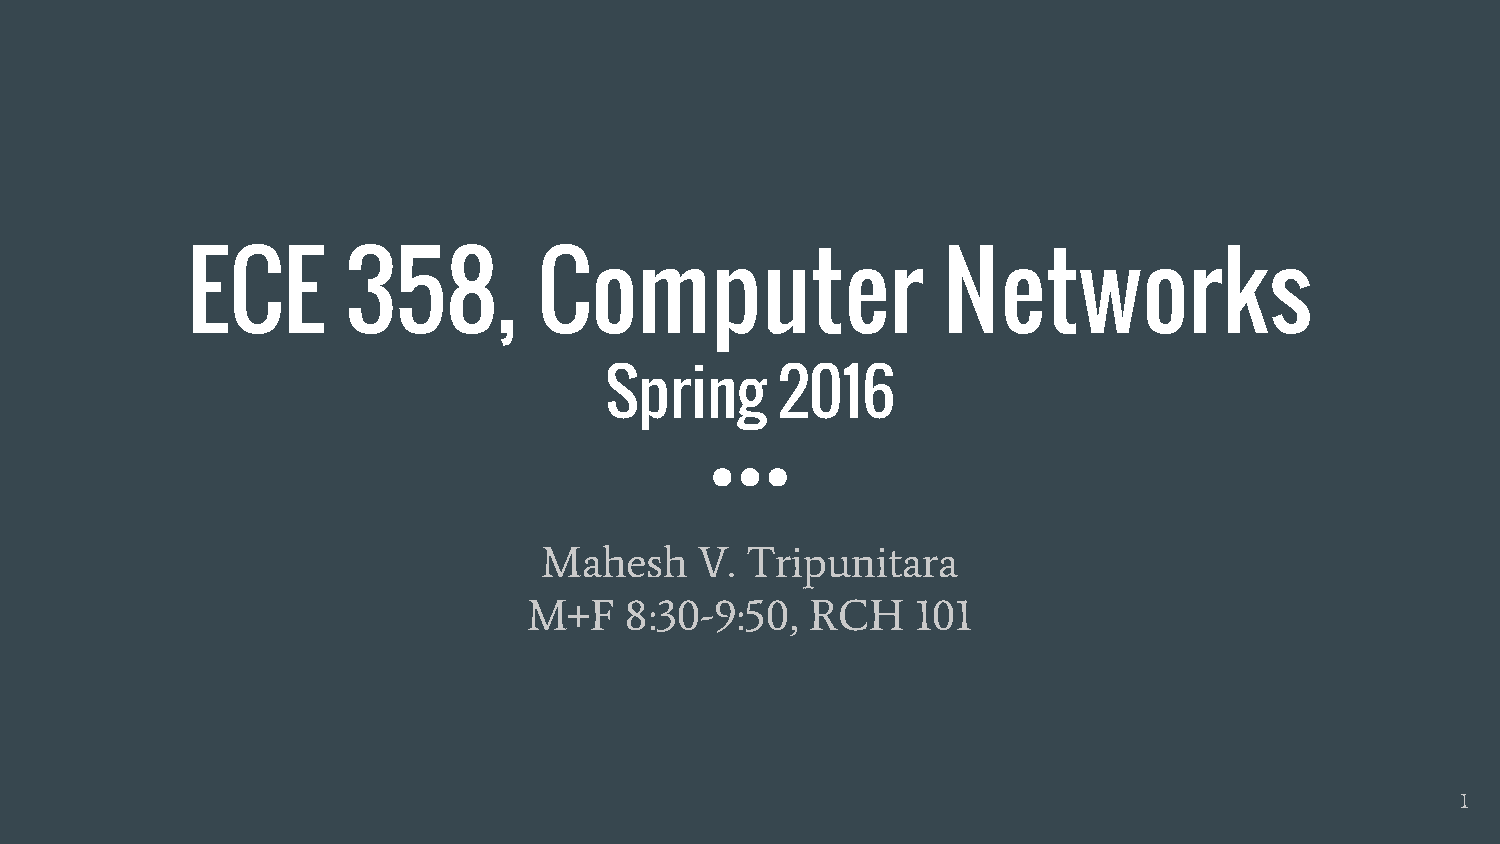
\includepdf[page=17]{slides.pdf}
\section{TCP/IP} % (fold)
\label{sec:tcp_ip}
The application top layer is usually the top tier layer, this can be an actual application or even a service like HTTP or DNS. The transport layer is rather important as it is where TCP lives. The network adjunct layer sets up shit (like security) for the network layer below it (includes ICMP which is essentially \texttt{ping}). Then is the network layer which is just IP. The lowest layer is the link layer but as with network there are some protocols in between. The link adjunct layer exists above the link layer and can be used to map addresses from IP to mac or some other form. 
% section tcp_ip (end)

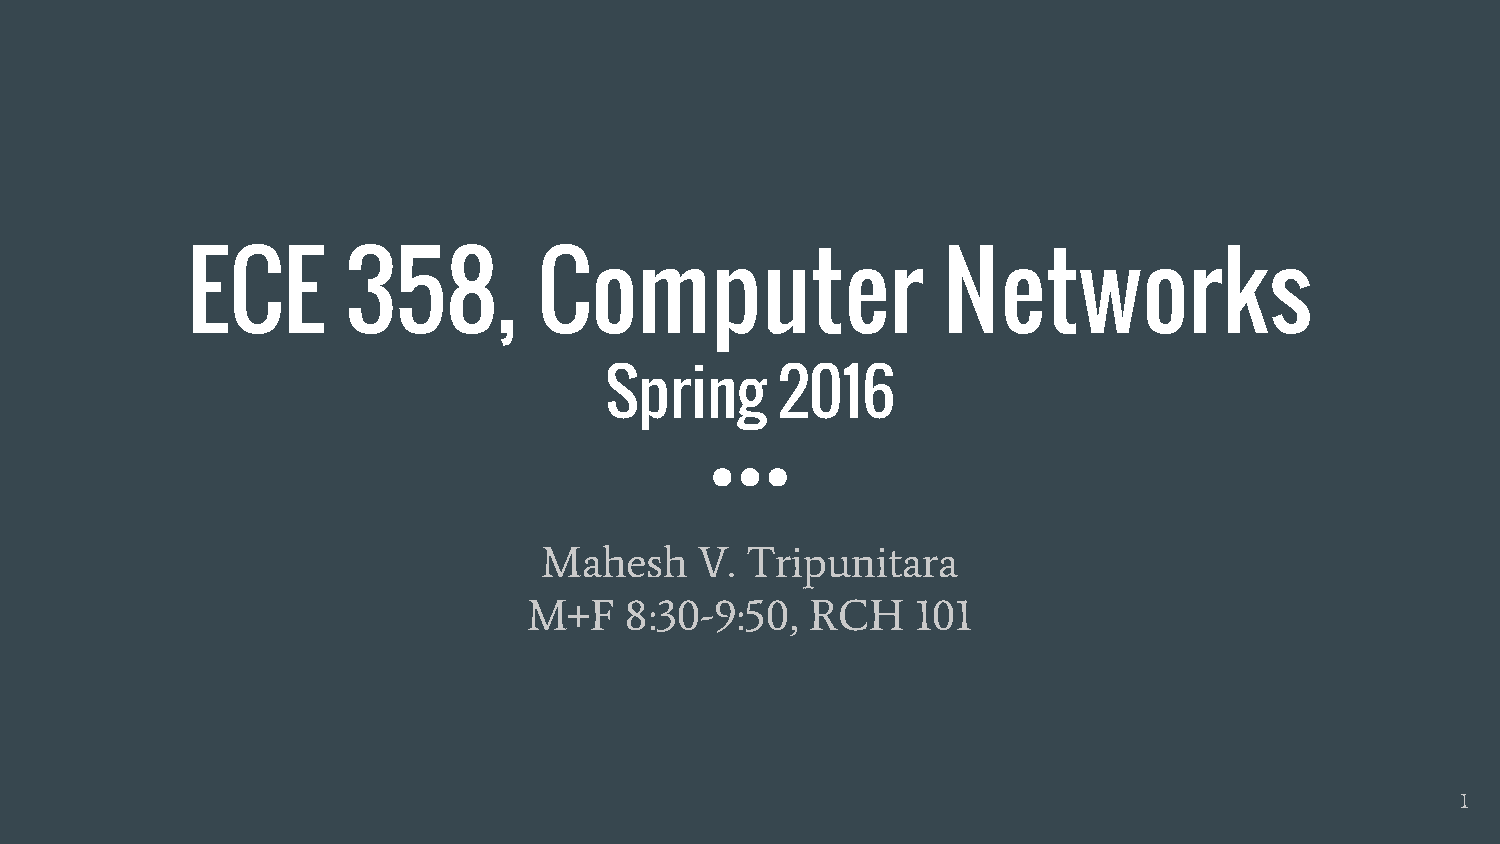
\includepdf[page=16]{slides.pdf}
\section{Ethernet Frames} % (fold)
\label{sec:ethernet_frames}
The ethernet standard is very different from the IP standard (the two evolved separately), for instance the ethernet standard has 2 more bytes. The ethernet address is allocated differently. For instance the first couple of bytes might represent the company that manufactured the device.  When you send a packet through a ethernet we need to know its ethernet address which is converted in the link adjunct layer.
% section ethernet_frames (end)

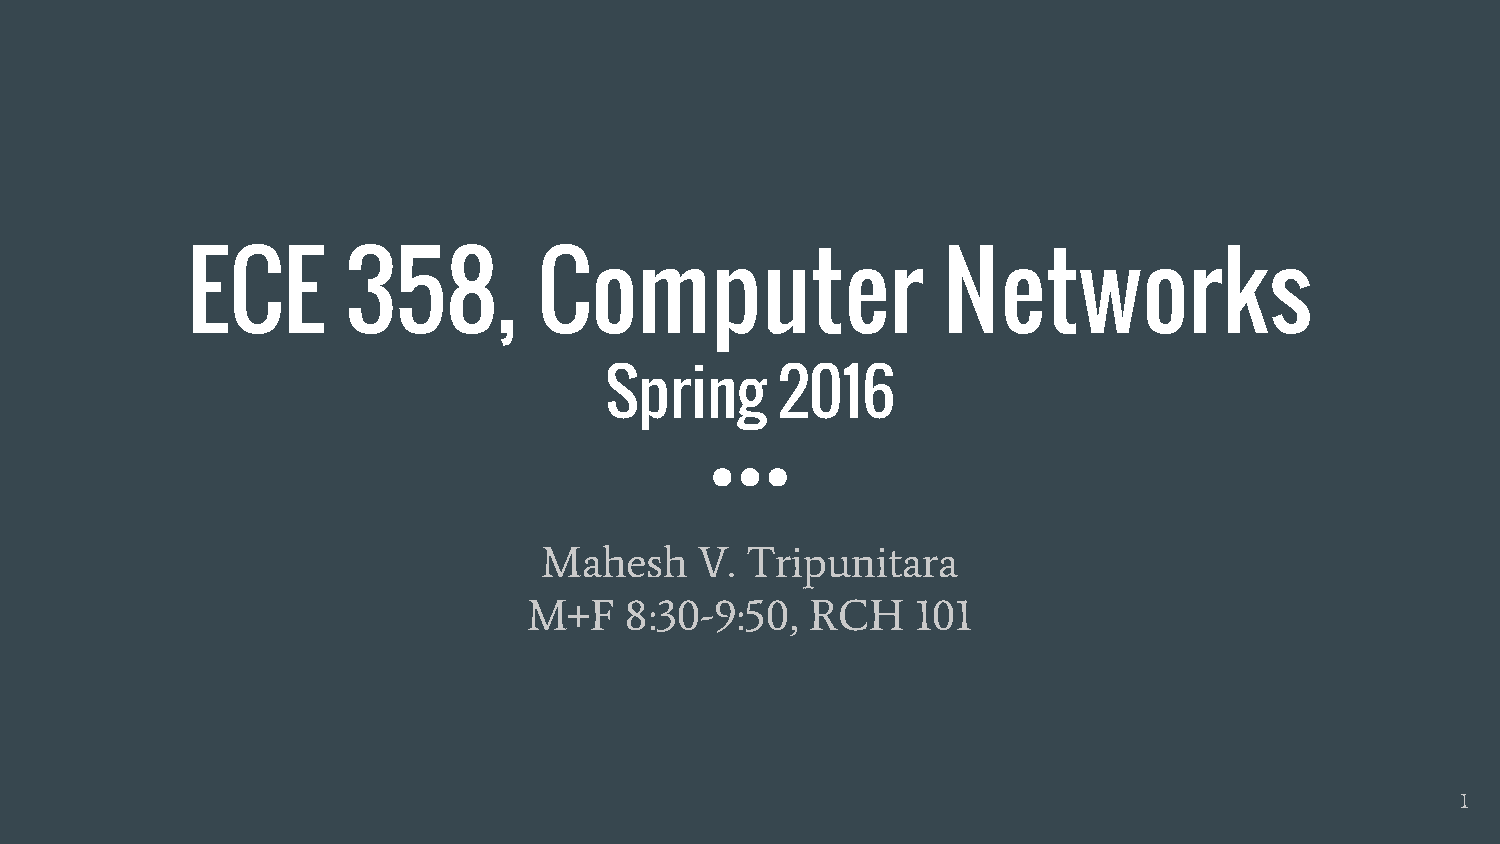
\includepdf[page=15]{slides.pdf}
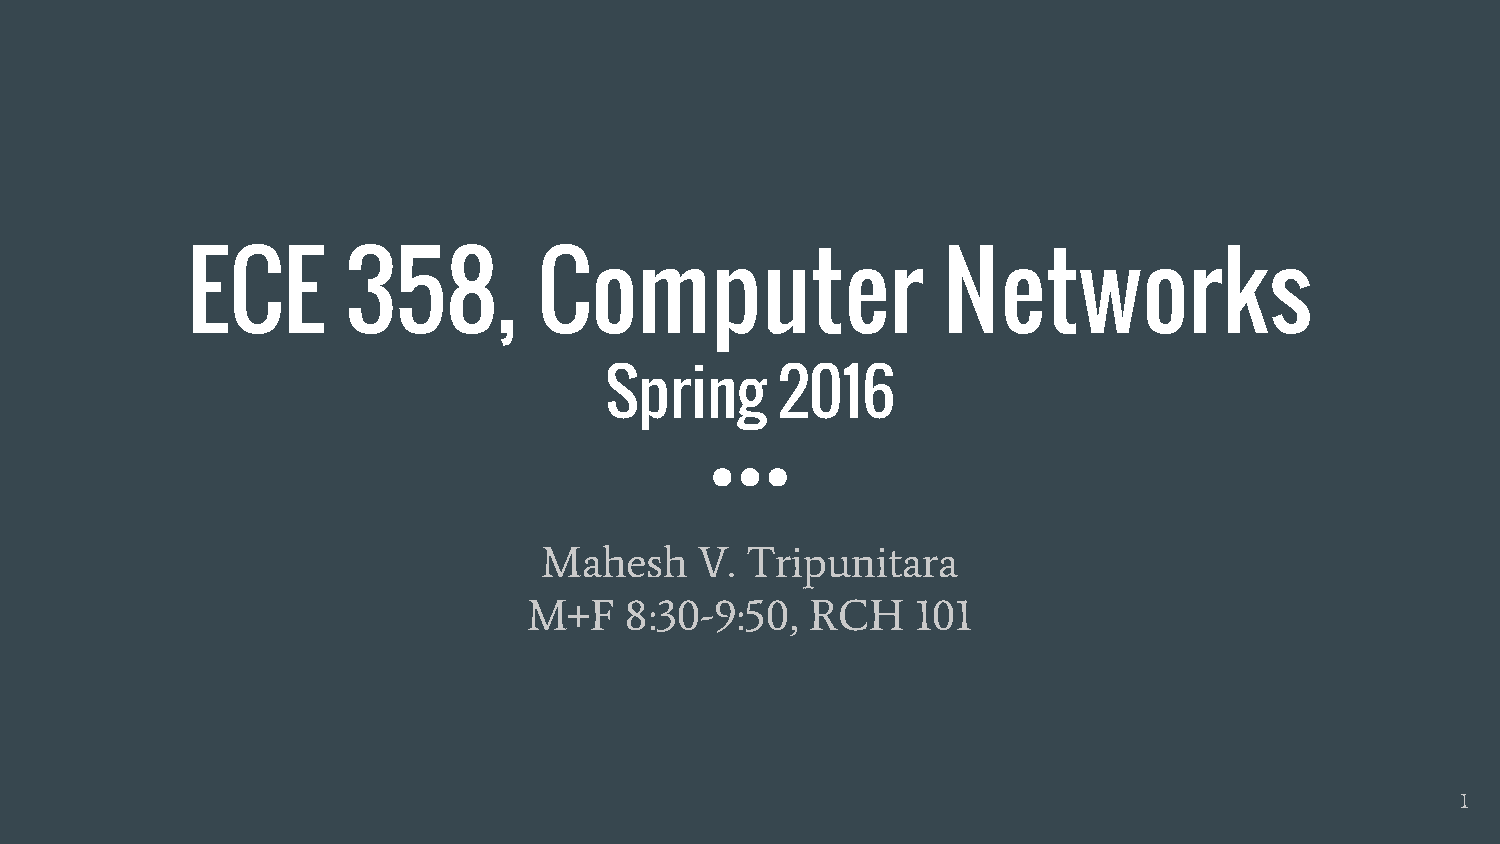
\includepdf[page=18]{slides.pdf}
\section{Encapsulation} % (fold)
\label{sec:encapsulation}
Each layer tacks on more information as the packet goes through, adding information needed by the next layer down. 

In the above example you start with UDP which then gets information added when it goes to TCP and again when it goes to IP and so on down the line as more information keeps being added until it gets to the link layer. 
% section encapsulation (end)

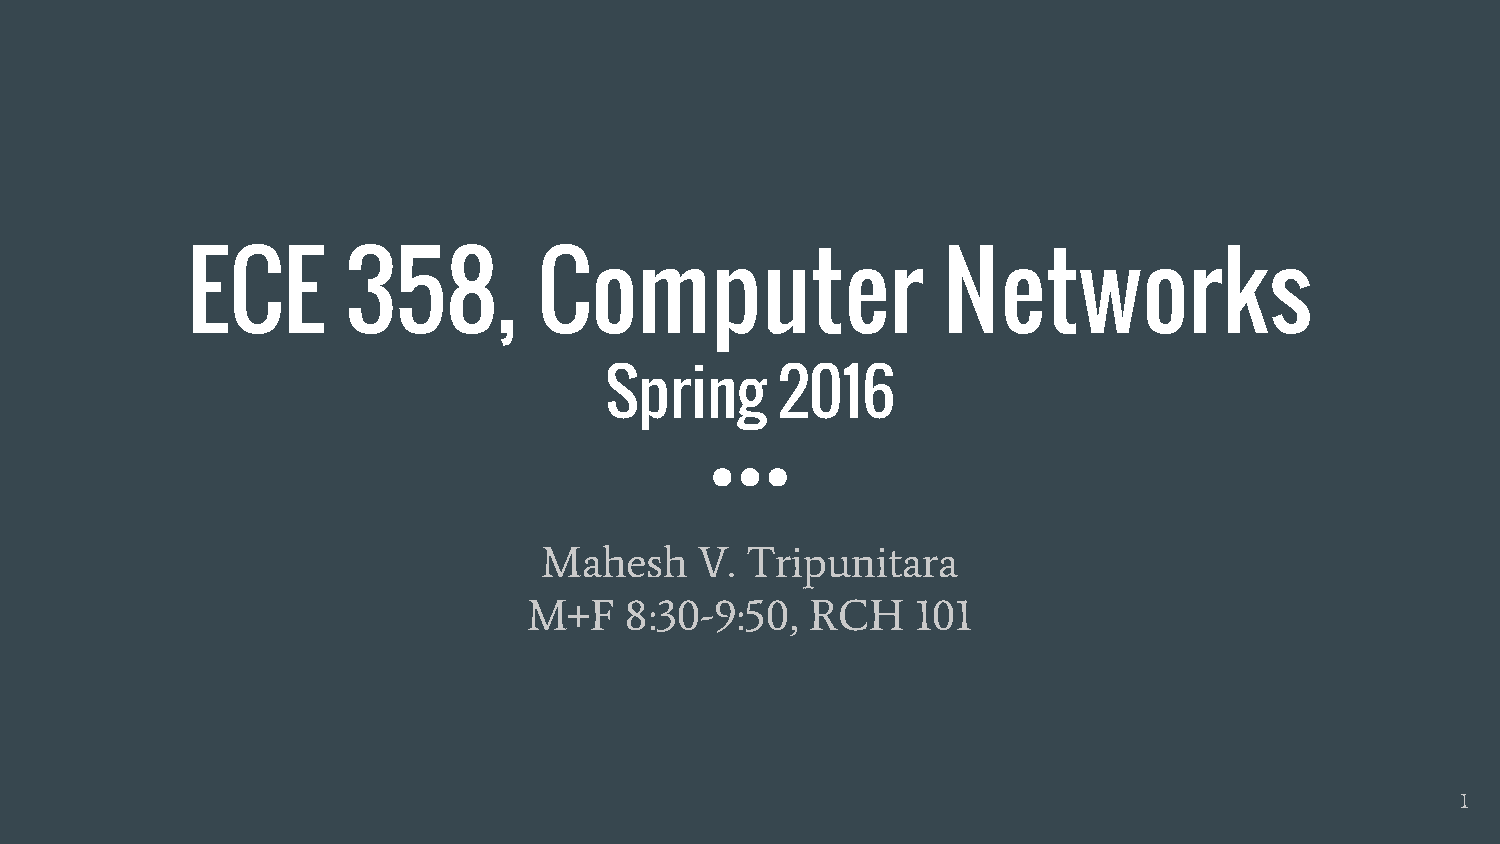
\includepdf[page=19]{slides.pdf}
This shows the layers that exist as they add information through encapsulation. This allows us to support all kinds of packets with various information. 

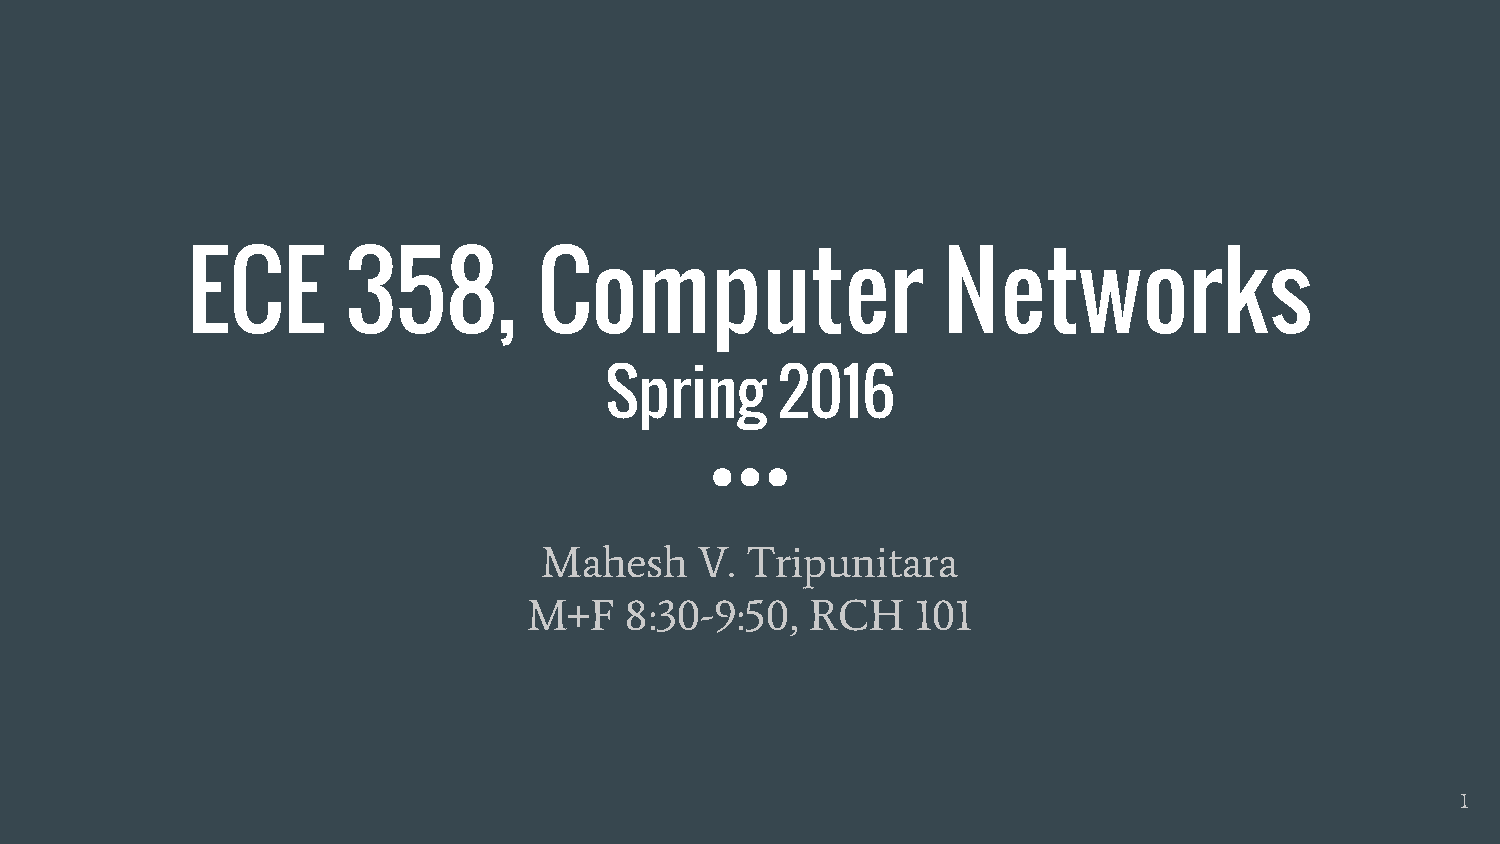
\includepdf[page=11]{slides.pdf}
This is the standard format of a packet. We have codes for each type of data in certain locations to tell how to handle that. As it goes down each layer looks ath athat protocol field and manipulates it as required. 


\end{document}